\documentclass[conference]{IEEEtran}
% Extrapolação de vista em elevação no 3DGS: diagnóstico e correções leves, com foco automotivo.
% Compilar com pdfLaTeX. Tabelas tab_*.tex e figuras em figs/ são geradas por
% experimentos/extrapolacao_sh/tabelas.py a partir dos resultados por vista.

\usepackage[utf8]{inputenc}
\usepackage[T1]{fontenc}
\usepackage[brazil]{babel}
\usepackage{cite}
\usepackage{amsmath,amssymb,amsfonts}
\usepackage{graphicx}
\usepackage{booktabs}
\usepackage{multirow}
\usepackage{textcomp}
\usepackage{xcolor}
\usepackage{url}
\usepackage[hidelinks]{hyperref}
\usepackage{icomma}

\newcommand{\pend}{\textcolor{red}{??}}

\begin{document}

\title{Reflexos Fora do Ângulo Filmado: 3DGS e Ref-Gaussian sob Cobertura Limitada de Elevação na Reconstrução de Veículos}

\author{\IEEEauthorblockN{João Pedro Maciel Pimenta}
\IEEEauthorblockA{\textit{Centro de Informática} \\
\textit{Universidade Federal de Pernambuco}\\
Recife, Brasil \\
jpmp3@cin.ufpe.br}
\and
\IEEEauthorblockN{Francisco Paulo Magalhães Simões}
\IEEEauthorblockA{\textit{Centro de Informática} \\
\textit{Universidade Federal de Pernambuco}\\
Recife, Brasil \\
fpms@cin.ufpe.br}
}

\maketitle

\begin{abstract}
Na reconstrução 3D de veículos, tanto a captura em volta de um carro para anúncios e inspeção quanto as gravações de direção usadas em simulação observam a cena numa faixa estreita de alturas de câmera, mas o modelo é consumido a partir de outros pontos de vista. Pintura, cromados e vidros tornam o problema mais difícil, porque são reflexivos. Este trabalho mede, num protocolo controlado, o que falha no 3D Gaussian Splatting (3DGS) e no Ref-Gaussian, um modelo de reflexão baseado em física, quando vistos acima da faixa filmada, e o que pode ser corrigido depois do treino. Usando o Shiny Blender, que tem imagens de referência de todos os ângulos, treinamos apenas com vistas abaixo de 25° (e de 15°) e avaliamos até 89°. O 3DGS perde 5,8~dB de PSNR de cima, e o mesmo 3DGS treinado com todas as alturas, sem as fotos avaliadas, recupera 7,2~dB nessas vistas; oráculos e a medida direta das normais mostram que sua geometria está errada em todas as alturas e é compensada pela cor. O Ref-Gaussian corrige a forma (11° de erro de normal de cima, contra 54°), mas sua vantagem cai de 2,1~dB na faixa para 0,3~dB de cima. Mostramos que o ambiente refletido de cima já havia sido observado no treino e, com oráculos por componente, que o que mais lhe falta de cima é precisão de forma: reajustar a geometria recupera 6,4~dB, contra 3,3~dB de toda a aparência, porque o reflexo amplifica o erro de normal que resta e a aparência, presa à física, não o compensa. Com as vistas de cima, o Ref-Gaussian ganha 11,4~dB e supera o 3DGS na mesma condição por 6,2~dB, e um controle por \textit{checkpoints} mostra que o ganho não vem das iterações. Avaliamos ainda correções leves sem retreino, entre elas uma projeção dos harmônicos esféricos com garantia de preservar as direções observadas, que roda em menos de 1~s em CPU: nenhuma recupera mais de 0,4~dB. Fora do ângulo filmado falta informação, não ajuste; discutimos em que cenário automotivo cada correção compensa e a extensão do protocolo a cenas dinâmicas de direção.
\end{abstract}


\begin{IEEEkeywords}
Gaussian Splatting, síntese de novas vistas, extrapolação de vista, harmônicos esféricos, reconstrução automotiva, compressão de modelos 3D.
\end{IEEEkeywords}

% =====================================================================
\section{Introdução}\label{sec:intro}

O 3D Gaussian Splatting (3DGS)~\cite{kerbl2023} reconstrói uma cena a partir de fotos com poses conhecidas e a renderiza em tempo real, com qualidade comparável à dos campos de radiância neurais (NeRF)~\cite{mildenhall2022nerf} e custo muito menor~\cite{fei2024survey}. A cena é um conjunto de Gaussianas 3D, cada uma com posição, forma, opacidade e uma cor que depende da direção de visão, descrita por harmônicos esféricos (SH) de grau 3: 16 coeficientes por canal de cor.

No domínio automotivo, essa representação aparece em dois usos. No primeiro, um veículo é fotografado ou filmado em volta para gerar uma visualização 3D destinada a anúncios ou inspeção. No segundo, gravações de direção são convertidas em cenas que um simulador renderiza a partir de trajetórias novas, para testar sistemas de percepção e condução~\cite{yang2023unisim,yan2024streetgs,zhou2024drivinggaussian,chen2025omnire}. Nos dois casos, as câmeras ocupam uma faixa estreita de alturas: na captura em volta do veículo, a câmera fica perto da altura dele; nas gravações de direção, as câmeras são fixas no carro~\cite{sun2020waymo}. O uso, porém, pede outros pontos de vista. O comprador gira o modelo para ver o teto, e o simulador precisa de mudanças de faixa ou de câmeras em outras alturas. Em cenas de direção, o \textit{benchmark} EUVS~\cite{han2025euvs} mostrou que o Gaussian Splatting perde muita qualidade em vistas extrapoladas e se ajusta demais às vistas de treino, e o FreeVS~\cite{wang2025freevs} relata o mesmo fora da trajetória gravada.

Capturar mais alturas nem sempre é possível. Uma gravação de direção é feita uma vez, e o simulador precisa justamente das vistas que ela não tem. Em serviços de anúncios, a captura é feita por terceiros, e filmar o teto de um veículo exige equipamento adicional, como bastões ou drones. Além disso, qualquer captura finita deixa direções sem observação. As perguntas práticas são, portanto, o que falha fora da faixa filmada, quanto vale a cobertura que falta e o que se pode corrigir depois do treino, a que custo.

Duas explicações concorrem. A geometria pode estar mal definida onde nenhuma câmera olhou. Ou a cor pode ser o problema, por dois motivos possíveis: um conjunto estreito de direções não determina os 16 coeficientes de SH (Seção~\ref{sec:metodo}), o que admitiria uma correção barata e sem treino; ou a aparência vista de cima simplesmente não está nas imagens, o que exigiria informação nova. Cada explicação leva a um remédio diferente. Este trabalho responde a quatro questões de pesquisa:
\begin{itemize}
\item \textbf{QP1.} Quanto se perde fora da faixa filmada, e como a perda depende da largura dessa faixa?
\item \textbf{QP2.} O erro de cima é de cor, de geometria ou da interação entre as duas?
\item \textbf{QP3.} Um modelo de reflexão baseado em física, o Ref-Gaussian~\cite{yao2025refgaussian}, extrapola melhor? Se não, que parte da sua aparência (material, iluminação do ambiente ou luz indireta) falha de cima?
\item \textbf{QP4.} Quanto recuperam correções leves, aplicadas a um modelo já treinado, e a que custo de tempo e armazenamento?
\end{itemize}

O caso automotivo torna a QP3 central. Pintura, cromados e vidros são superfícies reflexivas, justamente onde o 3DGS embute o reflexo na cor dependente de vista, e onde modelos como o Ref-Gaussian, que calculam o reflexo a partir da normal da superfície, de propriedades de material e de um mapa de ambiente compartilhado, prometem generalizar melhor.

Em dados reais essas questões não têm resposta, porque não existe imagem de referência do ângulo que faltou. Usamos então dados sintéticos como laboratório controlado: o Shiny Blender~\cite{verbin2022refnerf}, que inclui um carro entre seis objetos reflexivos, tem imagens de referência de todos os ângulos. Treinamos só com as vistas baixas e medimos o erro em função da elevação. As contribuições são:
\begin{itemize}
\item um protocolo controlado e reproduzível de extrapolação em elevação, com três grupos de avaliação, duas larguras de faixa e um modelo de referência treinado com cobertura completa;
\item uma decomposição do erro entre cor e geometria, por oráculos que reajustam só uma das partes e por uma medida direta da geometria contra silhuetas e normais de referência;
\item um diagnóstico do Ref-Gaussian sob cobertura limitada: geometria medida contra a referência, um teste de cobertura das direções refletidas e oráculos que reajustam separadamente material, mapa de ambiente e luz indireta, com controle do efeito do número de iterações;
\item uma análise do condicionamento dos SH sob faixas estreitas e uma projeção sem treino, com garantia de alterar pouco as direções observadas;
\item uma comparação de custo e qualidade entre correções leves existentes (truncamento e redução adaptativa de grau dos SH), a projeção e o ganho de capturar de cima;
\item a aplicação a um veículo real e o código aberto, incluindo uma ferramenta que corrige um modelo \texttt{.ply} em menos de 1~s em CPU.
\end{itemize}

\begin{figure}[t]
\centering
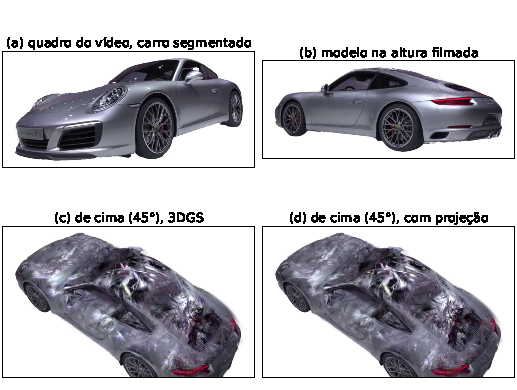
\includegraphics[width=\columnwidth]{figs/teaser.pdf}
\caption{Porsche 911 reconstruído por um pipeline de produção de anúncios a partir de um vídeo com câmeras entre 0,4° e 3,8° de elevação. Na altura filmada (b), o modelo é fiel ao vídeo (a). A 45° (c), o teto e o capô mostram manchas e reflexos que não existem. A projeção dos SH no subespaço observado (d) quase não muda a imagem.}
\label{fig:teaser}
\end{figure}


% =====================================================================
\section{Trabalhos Relacionados}\label{sec:relacionados}

\textbf{Cor dependente de vista e reflexos.} Os SH vêm da computação gráfica, onde representam iluminação e transporte de luz de baixa frequência~\cite{ramamoorthi2001irradiance,sloan2002prt}. PlenOctrees~\cite{yu2021plenoctrees} e Plenoxels~\cite{fridovich2022plenoxels} os adotaram para guardar a cor de campos de radiância sem rede neural, e o 3DGS~\cite{kerbl2023} herdou essa escolha. Gaussianas esféricas anisotrópicas~\cite{yang2024spec} e modelos de reflexão física melhoram reflexos nítidos. Nos campos neurais, o Ref-NeRF~\cite{verbin2022refnerf} parametriza a cor pela direção refletida, o NeRO~\cite{liu2023nero} recupera geometria e BRDF de objetos reflexivos e o NeRF-Casting~\cite{verbin2024nerfcasting} traça raios refletidos na própria cena. No 3DGS, o GaussianShader~\cite{jiang2024gshader} aplica uma função de sombreamento com a normal dada pelo eixo mais curto de cada Gaussiana, o 3DGS-DR~\cite{ye2024gsdr} adia o cálculo do reflexo para o espaço da imagem e o Ref-Gaussian~\cite{yao2025refgaussian}, construído sobre Gaussianas 2D~\cite{huang2024gs2d}, combina renderização baseada em física com reflexos entre partes do objeto. Esses métodos são avaliados em vistas de teste próximas das de treino; nenhum deles mede o que acontece longe delas.

\textbf{Poucas vistas e vistas extrapoladas.} Com poucas imagens, NeRF e 3DGS se ajustam demais às vistas de treino. RegNeRF~\cite{niemeyer2022regnerf} e FreeNeRF~\cite{yang2023freenerf} regularizam geometria e frequência durante o treino; FSGS~\cite{zhu2024fsgs} e DNGaussian~\cite{li2024dngaussian} usam profundidade monocular. Para vistas distantes, a linha atual usa modelos gerativos pré-treinados: ReconFusion~\cite{wu2024reconfusion} e CAT3D~\cite{gao2024cat3d} geram vistas novas por difusão, GaussianObject~\cite{yang2024gaussianobject} completa objetos a partir de quatro fotos, ViewExtrapolator~\cite{liu2024viewextrapolator} refina vistas extrapoladas com um modelo de vídeo e Difix3D+~\cite{wu2025difix3d} corrige artefatos com difusão de um passo. Esses métodos recuperam geometria e cor, mas exigem retreino, GPUs com muita memória ou modelos de bilhões de parâmetros, e podem inventar detalhes, o que é indesejável em inspeção.

\textbf{Reconstrução para direção autônoma.} UniSim~\cite{yang2023unisim} reconstrói gravações de direção para simulação em malha fechada. Street Gaussians~\cite{yan2024streetgs}, DrivingGaussian~\cite{zhou2024drivinggaussian} e OmniRe~\cite{chen2025omnire} representam o fundo e os agentes dinâmicos com Gaussianas; o Street Gaussians modela a aparência dos veículos com SH que variam no tempo. Na mesma linha das representações dinâmicas gerais~\cite{wu2024gs4d}, todos herdam a cor por SH do 3DGS. EUVS~\cite{han2025euvs} e FreeVS~\cite{wang2025freevs} mostram que a qualidade cai fora da trajetória gravada, mas não separam as causas dessa queda.

\textbf{Redução dos SH.} Trabalhos de compressão mostraram que muitos coeficientes de SH são dispensáveis: o LightGaussian~\cite{fan2024lightgaussian} reduz o grau por destilação e Papantonakis et al.~\cite{papantonakis2024reducing} escolhem o grau por Gaussiana. O objetivo deles é memória dentro da faixa observada; aqui eles servem como correções leves de referência fora dela.

\textbf{Avaliação com cobertura realista.} Gao et al.~\cite{gao2022dycheck} mostraram, para cenas dinâmicas, que protocolos comuns dão ao modelo mais pontos de vista do que uma captura casual daria. Simuladores como o CARLA~\cite{dosovitskiy2017carla} fornecem cenas automotivas com referência exata de qualquer ponto de vista. Este trabalho segue essa linha num caso estático e controlado: a cobertura em elevação.

\textbf{Posicionamento.} A Tabela~\ref{tab:relacionados} resume as diferenças. Os trabalhos acima propõem soluções e medem o resultado final. Este trabalho mede onde está o erro, separando cor de geometria, e compara correções de custos muito diferentes no mesmo protocolo, o que permite escolher entre elas conforme o cenário de uso.

\begin{table}[t]
\centering
\caption{Trabalhos que tratam vistas pouco ou nada observadas. ``Treino'': exige treinar ou retreinar a cena; ``Prior'': conhecimento externo usado; ``Geo./Cor'': o que a técnica corrige.}
\label{tab:relacionados}
\setlength{\tabcolsep}{3pt}
\footnotesize
\begin{tabular}{l c c c c}
\toprule
Trabalho & Treino & Prior & Geo. & Cor \\
\midrule
RegNeRF, FreeNeRF~\cite{niemeyer2022regnerf,yang2023freenerf} & sim & não & sim & parcial \\
FSGS, DNGaussian~\cite{zhu2024fsgs,li2024dngaussian} & sim & profund. & sim & parcial \\
ReconFusion, CAT3D~\cite{wu2024reconfusion,gao2024cat3d} & sim & difusão & sim & sim \\
GaussianObject~\cite{yang2024gaussianobject} & sim & difusão & sim & sim \\
ViewExtrapolator~\cite{liu2024viewextrapolator} & não$^\dagger$ & vídeo & sim & sim \\
Difix3D+~\cite{wu2025difix3d} & opcional & difusão & sim & sim \\
Ref-Gaussian, GShader~\cite{yao2025refgaussian,jiang2024gshader} & sim & física & sim & reflexo \\
Cenas de direção~\cite{yan2024streetgs,zhou2024drivinggaussian,chen2025omnire} & sim & LiDAR & sim & não \\
FreeVS~\cite{wang2025freevs} & sim & difusão & sim & sim \\
Redução de SH~\cite{fan2024lightgaussian,papantonakis2024reducing} & sim & não & não & não \\
\midrule
\textbf{Este trabalho} & \textbf{não} & \textbf{não} & diagnóst. & parcial \\
\bottomrule
\end{tabular}

\vspace{2pt}
{\scriptsize $^\dagger$ inferência com modelo de vídeo de bilhões de parâmetros a cada nova vista.}
\end{table}


% =====================================================================
\section{Método}\label{sec:metodo}

\subsection{Cor por harmônicos esféricos}

No 3DGS, a cor da Gaussiana $i$ vista na direção unitária $\mathbf{d}$ (da câmera para a Gaussiana) é, por canal,
\begin{equation}
c_i(\mathbf{d}) = \mathbf{y}(\mathbf{d})^\top \mathbf{a}_i + 0{,}5,
\end{equation}
em que $\mathbf{y}(\mathbf{d}) \in \mathbb{R}^{16}$ reúne os SH reais até o grau 3 e $\mathbf{a}_i$ são os coeficientes aprendidos. O primeiro termo, $y_0$, é constante: é a cor média (``DC''). Os outros 15 descrevem como a cor muda com a direção.

\subsection{O que as câmeras de treino determinam}

Seja $\{\mathbf{d}_{ij}\}$ o conjunto de direções em que a Gaussiana $i$ aparece nas câmeras de treino $j$, com pesos $w_{ij} \ge 0$ que medem quanto ela contribui para os pixels da vista $j$. A perda de treino só observa $c_i$ nessas direções. Definimos a matriz de Gram
\begin{equation}
G_i = \frac{\sum_j w_{ij}\, \mathbf{y}(\mathbf{d}_{ij})\, \mathbf{y}(\mathbf{d}_{ij})^\top}{\sum_j w_{ij}} \in \mathbb{R}^{16\times 16}.
\end{equation}
A variação quadrática média da cor nas direções observadas, quando os coeficientes mudam de $\mathbf{a}$ para $\mathbf{a}+\boldsymbol{\delta}$, é $\boldsymbol{\delta}^\top G_i \boldsymbol{\delta}$. Se $\mathbf{v}$ é um autovetor de $G_i$ com autovalor próximo de zero, somar $\alpha\mathbf{v}$ aos coeficientes não muda nenhuma vista de treino, mas pode mudar muito as vistas de fora. O treino não tem como fixar essas combinações; o valor delas resulta da inicialização, do ruído do otimizador e do ajuste a ruído das imagens.

A Fig.~\ref{fig:espectro} mostra o espectro de $G$ para faixas de elevação com todos os azimutes, como numa volta completa. Na esfera inteira, os 16 autovalores são iguais. Na faixa de um veículo real filmado entre 0,4° e 3,8°, 9 dos 16 ficam abaixo de 1\% do maior e 4 abaixo de $10^{-4}$. Mesmo no hemisfério superior inteiro restam 3 direções mal determinadas. Isso explica o resultado da Tabela~\ref{tab:treino}: mais iterações ou outra estratégia de densificação~\cite{kheradmand2024mcmc} não acrescentam informação sobre direções que nenhuma imagem mostra.

\begin{figure}[t]
\centering
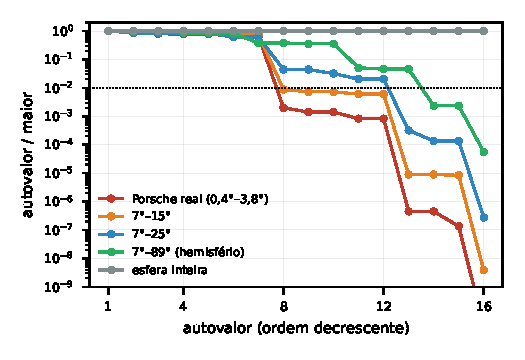
\includegraphics[width=\columnwidth]{figs/espectro_gram.pdf}
\caption{Autovalores da matriz de Gram dos SH de grau 3 (normalizados pelo maior) para direções de uma volta completa em diferentes faixas de elevação. Autovalores pequenos correspondem a combinações de coeficientes que não alteram nenhuma vista filmada.}
\label{fig:espectro}
\end{figure}

\subsection{Projeção no subespaço observado}

Propomos substituir, depois do treino, os coeficientes de cada Gaussiana pelos de menor norma que reproduzem a mesma cor nas direções observadas:
\begin{equation}
\begin{split}
\mathbf{a}_i' &= \arg\min_{\mathbf{a}}\; (\mathbf{a}-\mathbf{a}_i)^\top G_i (\mathbf{a}-\mathbf{a}_i) + \lambda\, \mathbf{a}^\top L\, \mathbf{a}\\
&= (G_i + \lambda L)^{-1} G_i\, \mathbf{a}_i,
\end{split}
\label{eq:proj}
\end{equation}
com $L = \mathrm{diag}(0, 1, \dots, 1)$: a cor média nunca é penalizada. A solução se aplica aos três canais de cor e tem duas propriedades.

\textit{(i) Altera pouco as direções observadas.} Com $\mathbf{e} = \mathbf{a}_i - \mathbf{a}_i'$, decompondo no problema generalizado de autovalores $L\mathbf{v}=\mu G_i \mathbf{v}$, cada componente é multiplicado por $\lambda\mu/(1+\lambda\mu)$ e, como $(1+x)^2 \ge 4x$,
\begin{equation}
\mathbf{e}^\top G_i\, \mathbf{e} \;\le\; \frac{\lambda}{4}\, \mathbf{a}_i^\top L\, \mathbf{a}_i .
\end{equation}
A mudança quadrática média da cor nas direções de treino é no máximo $\lambda/4$ vezes a energia dos termos não constantes. A garantia vale para as direções de treino, e não necessariamente para direções intermediárias entre elas.

\textit{(ii) Remove o que não foi observado.} Quando $L$ comuta com $G_i$, cada componente na base de autovetores de $G_i$ é multiplicado por $\sigma/(\sigma+\lambda)$, o filtro de Tikhonov~\cite{tikhonov1963}: direções bem observadas ($\sigma \gg \lambda$) ficam intactas e as não observadas ($\sigma \ll \lambda$) são zeradas. Fora da faixa filmada, a cor tende ao valor mais simples compatível com o que foi visto. Uma Gaussiana que nunca apareceu em nenhuma câmera fica só com a cor média.

\subsection{Duas formas de obter as direções observadas}

\textbf{Global.} Uma única matriz para a cena inteira, com as direções de uma volta completa na faixa de elevação das câmeras (com 5° de margem). Custa uma multiplicação $16\times16$ por Gaussiana e dispensa GPU e imagens: basta saber a faixa de elevação. Ignora a paralaxe (a direção da câmera muda conforme a posição da Gaussiana) e a oclusão.

\textbf{Por visibilidade.} Para cada Gaussiana, usamos as direções reais $\mathbf{d}_{ij} = (\boldsymbol{\mu}_i - \mathbf{o}_j)/\lVert\boldsymbol{\mu}_i - \mathbf{o}_j\rVert$ até cada câmera de treino $\mathbf{o}_j$, com peso $w_{ij} = \sum_{p} \alpha_i(p)\, T_i(p)$: a soma, nos pixels $p$ da vista $j$, da opacidade da Gaussiana vezes a transmitância acumulada até ela. Esse peso já conta oclusão e enquadramento, e sai do próprio rasterizador: renderizando com cor constante igual a 1 e retropropagando a soma da imagem, o gradiente em relação à cor de cada Gaussiana é exatamente $w_{ij}$. O custo é uma renderização com retropropagação por câmera de treino e um sistema $16\times16$ por Gaussiana, resolvidos em lote na GPU.

\subsection{Correções leves de referência}\label{sec:leves}

Comparamos a projeção com correções existentes que também atuam sobre os SH de um modelo já treinado, sem retreino:
\begin{itemize}
\item \textbf{Truncamento de grau} (grau 0, 1 ou 2): zera os SH acima do grau escolhido. É o que fazem visualizadores leves e formatos compactos, e o grau 0 elimina toda a dependência de vista.
\item \textbf{Grau adaptativo por Gaussiana}, no espírito de Papantonakis et al.~\cite{papantonakis2024reducing}: para cada Gaussiana, escolhemos o menor grau $\ell$ tal que a cor nas direções observadas muda menos que $\tau$, isto é, $\sqrt{\tfrac{1}{3}\sum_c \boldsymbol{\delta}_{\ell,c}^\top G_i\, \boldsymbol{\delta}_{\ell,c}} \le \tau$, em que $\boldsymbol{\delta}_{\ell,c}$ são os coeficientes descartados no canal $c$. Usamos $\tau = 0{,}01$ (escala de cor de 0 a 1).
\item \textbf{Projeção seguida do grau adaptativo}: a projeção zera o que nenhuma câmera viu, e o grau adaptativo descarta esses coeficientes do armazenamento.
\end{itemize}
O armazenamento por Gaussiana, em precisão simples, é $4\,(11 + 3K)$ bytes, com $K$ coeficientes de SH por canal: 204 bytes no grau 3 e 56 bytes no grau 0.

% =====================================================================
\section{Protocolo Experimental}\label{sec:exp}

\textbf{Dados sintéticos.} O Shiny Blender~\cite{verbin2022refnerf} tem seis objetos com materiais reflexivos (\textit{ball}, \textit{car}, \textit{coffee}, \textit{helmet}, \textit{teapot} e \textit{toaster}), imagens de 800$\times$800 px, 100 vistas de treino espalhadas no hemisfério superior (de 7° a 89° de elevação; na \textit{ball}, na esfera inteira) e 200 vistas de teste numa espiral entre 7° e 47°. Treinamos só com as vistas de treino abaixo de 25° de elevação, de 26 a 37 vistas por cena, imitando uma captura feita em volta do objeto, numa altura só. As vistas de treino não usadas cobrem até 89°, quase a vista de topo. Separamos três grupos, todos inéditos para o modelo:
\begin{itemize}
\item \textbf{dentro da faixa}: vistas de teste abaixo de 25° (interpolação);
\item \textbf{acima}: vistas de teste entre 25° e 47° (extrapolação moderada);
\item \textbf{de cima}: vistas de treino não usadas, entre 50° e 89°.
\end{itemize}
A Fig.~\ref{fig:protocolo} mostra os grupos numa cena. As vistas de treino não usadas entre 25° e 50° ficam de fora, para que o grupo ``acima'' tenha só vistas de teste. Para medir o efeito da largura da faixa (QP1), repetimos o experimento com treino abaixo de 15°. Como referência de cobertura completa, treinamos o mesmo 3DGS com as 100 vistas de treino. Como as vistas de cima fazem parte do treino desse modelo, treinamos também uma versão com todas as alturas \emph{sem as fotos avaliadas}: das 100 vistas de treino, separamos, alternadamente por elevação, metade das vistas acima de 50° e as vistas usadas na demonstração interativa (de 22 a 24 por cena; 9 no \textit{ball}). As vistas restantes cobrem de 7° a 86° (78° no \textit{teapot} e 68° no \textit{ball}), e as separadas são inéditas para todos os modelos comparados. A Tabela~\ref{tab:modelos} lista todos os modelos avaliados.

\begin{table}[t]
\centering
\caption{Modelos avaliados. ``Faixa'': só as vistas de treino abaixo de 25° (de 26 a 37 por cena); ``completo'': as 100 vistas de treino, de todas as alturas. Tempo médio de treino por cena numa RTX 4050 de 6~GB. As correções leves são aplicadas ao 3DGS da faixa, sem retreino.}
\label{tab:modelos}
\setlength{\tabcolsep}{2.5pt}
\footnotesize
\begin{tabular}{l l c c r}
\toprule
Modelo & Implementação & Vistas & Iter. & Tempo \\
\midrule
3DGS, faixa & gsplat 1.5.3, SH grau 3 & faixa & 30 mil & 20 min \\
3DGS, completo & gsplat 1.5.3, SH grau 3 & 100 & 30 mil & 20 min \\
3DGS, todas$^\ast$ & gsplat 1.5.3, SH grau 3 & 76--91 & 30 mil & 20 min \\
Ref-Gaussian, faixa & oficial, crono.\ escalado & faixa & 28 mil & 47 min \\
Ref-Gaussian, completo & oficial, crono.\ original & 100 & 50 mil & 106 min$^\dagger$ \\
Ref-Gaussian, todas$^\ast$ & oficial, crono.\ escalado & 78 & 28 mil & 52 min \\
Correções leves & sobre o 3DGS da faixa & -- & -- & $\le$1,3 s \\
\bottomrule
\end{tabular}

\vspace{2pt}
{\scriptsize $^\ast$ todas as alturas, sem as fotos avaliadas. $^\dagger$ medido no \textit{toaster}, fora do contêiner usado nos demais treinos.}
\end{table}


\begin{figure}[t]
\centering
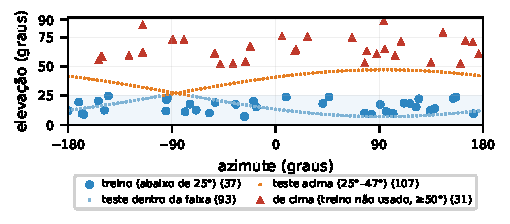
\includegraphics[width=\columnwidth]{figs/protocolo.pdf}
\caption{Câmeras da cena \textit{car} por azimute e elevação: treino abaixo de 25°, vistas de teste na espiral e vistas de cima usadas só na avaliação.}
\label{fig:protocolo}
\end{figure}

\textbf{Oráculos.} Para separar cor de geometria (QP2), reajustamos só uma parte do modelo treinado, com a mesma perda do treino (3000 passos de Adam), usando as vistas de \emph{avaliação} de um grupo. É um procedimento deliberadamente privilegiado: o resultado é o teto do que uma correção restrita àquela parte poderia atingir, e não um método. O oráculo de cor reajusta todos os SH com a geometria congelada; uma variante reajusta só a cor constante, zerando os termos direcionais; o oráculo de geometria reajusta posições, escalas, rotações e opacidades com os SH congelados, com as taxas de aprendizado do treino original. Para não medir memorização, o ajuste usa as vistas de índice par do grupo e a avaliação usa as de índice ímpar. Num controle mais rigoroso, o ajuste usa só as vistas de um lado do objeto (azimute negativo) e a avaliação, as do outro lado.

\textbf{Geometria.} Medimos a geometria diretamente, sem passar pela cor, contra a silhueta e o mapa de normais de referência de cada vista (Seção~\ref{sec:geometria}).

\textbf{Ref-Gaussian.} Para a QP4, treinamos o Ref-Gaussian~\cite{yao2025refgaussian} com o código oficial nas mesmas vistas de treino de três cenas (\textit{car}, \textit{helmet} e \textit{toaster}) e o avaliamos nas mesmas vistas. O cronograma do método foi escalado proporcionalmente para 28 mil iterações. Com 30 mil iterações, o início da luz indireta coincide com um reinício de opacidade, a malha usada no traçado de raios não é extraída e o treino falha; 28 mil evita a coincidência. Como referência, usamos também modelos do Ref-Gaussian treinados com o hemisfério todo e o cronograma original de 50 mil iterações.

\textbf{Escolha dos parâmetros.} O 3DGS usa a configuração padrão do artigo original~\cite{kerbl2023}: 30 mil iterações e SH de grau 3. O Ref-Gaussian completo usa o cronograma oficial de 50 mil iterações, com o qual nossa replicação atinge 34,5~dB de PSNR médio nas seis cenas do Shiny Blender, contra 35,0~dB relatados pelos autores. O Ref-Gaussian da faixa usa 28 mil iterações, para que a comparação com o 3DGS, que usa 30 mil, não favoreça o método mais caro; todas as fases do cronograma foram escaladas na mesma proporção. Como o modelo completo tem mais iterações que o da faixa, avaliamos também seus \textit{checkpoints} de 30 e 40 mil iterações (Seção~\ref{sec:refgs}), para separar o efeito das iterações do efeito das vistas. Nas correções, $\lambda = 10^{-2}$ é o menor valor que atua sem custar qualidade na faixa (Tabela~\ref{tab:lambda}), e $\tau = 0{,}01$ corresponde a cerca de 2,5 níveis de cor em 8 bits.

\textbf{Custo.} Medimos o tempo de cada correção na mesma GPU e o armazenamento resultante pela fórmula da Seção~\ref{sec:leves}. A projeção global também foi medida em CPU, aplicada diretamente a um arquivo \texttt{.ply}.

\textbf{Implementação.} Usamos o 3DGS da biblioteca gsplat~1.5.3~\cite{ye2025gsplat} com os hiperparâmetros do artigo original: 30 mil iterações, densificação até a metade do treino, SH de grau 3 liberado gradualmente, 100 mil pontos iniciais aleatórios e fundo branco. Na gsplat~1.5.3 o reinício periódico de opacidade nunca é acionado, por um erro de precedência de operadores; nós o reimplementamos no laço de treino. Medimos PSNR, SSIM~\cite{wang2004ssim} e LPIPS-VGG~\cite{zhang2018lpips} na imagem inteira, com intervalos de confiança por \textit{bootstrap}~\cite{efron1993bootstrap}. Os experimentos rodam numa RTX~4050 de 6~GB.

\textbf{Veículo real.} Usamos capturas de um pipeline de produção de anúncios 3D de veículos. O pipeline extrai quadros nítidos do vídeo, segmenta o veículo com Mask R-CNN~\cite{he2017maskrcnn} refinado pelo SAM~\cite{kirillov2023sam}, estima as poses com o COLMAP~\cite{schonberger2016colmap} usando só pontos do veículo e treina o 3DGS só no veículo, com fundo aleatório a cada passo. A Tabela~\ref{tab:treino} usa esse pipeline para dois carros. Num Porsche 911 filmado com câmeras entre 0,4° e 3,8°, comparamos o modelo antes e depois da projeção global.

\begin{table}[t]
\centering
\caption{Veículos reais do pipeline de anúncios: treinar mais ou trocar a estratégia de densificação quase não muda a qualidade nas vistas de validação (PSNR medido só nos pixels do carro). As variantes reutilizam os mesmos quadros, máscaras e poses do COLMAP.}
\label{tab:treino}
\setlength{\tabcolsep}{3pt}
\footnotesize
\begin{tabular}{l l c c c c c}
\toprule
Carro & Variante & PSNR & Pior & SSIM & LPIPS & Treino \\
\midrule
\multirow{3}{*}{Ford GT} & 30k it., 1280 px & 22,24 & 15,16 & 0,946 & 0,094 & 22 min \\
 & 60k it., 1600 px & 22,23 & 15,13 & 0,948 & 0,097 & 85 min \\
 & 60k + MCMC~\cite{kheradmand2024mcmc} & 22,32 & 15,06 & 0,950 & 0,097 & 129 min \\
\midrule
\multirow{3}{*}{Porsche 911} & 30k it., 1280 px & 26,11 & 20,93 & 0,960 & 0,078 & 23 min \\
 & 60k it., 1600 px & 26,28 & 20,73 & 0,963 & 0,078 & 90 min \\
 & 60k + MCMC~\cite{kheradmand2024mcmc} & 26,37 & 20,49 & 0,964 & 0,082 & 130 min \\
\bottomrule
\end{tabular}
\end{table}


% =====================================================================
\section{Resultados}\label{sec:resultados}

\begin{table*}[t]
\centering
\caption{Média nas 6 cenas do Shiny Blender, treino só com vistas abaixo de 25°. Faixa e acima: vistas de teste; de cima: vistas de treino não usadas, entre 50° e 89°. As correções são aplicadas ao mesmo modelo treinado, sem novo treino. Em negrito, o melhor entre as variantes desse modelo.}
\label{tab:principal25}
\begin{tabular}{l ccc ccc ccc}
\toprule
 & \multicolumn{3}{c}{Dentro da faixa ($<25$°)} & \multicolumn{3}{c}{Acima (25°--47°)} & \multicolumn{3}{c}{De cima (50°--89°)} \\
\cmidrule(lr){2-4}\cmidrule(lr){5-7}\cmidrule(lr){8-10}
Variante & PSNR$\uparrow$ & SSIM$\uparrow$ & LPIPS$\downarrow$ & PSNR$\uparrow$ & SSIM$\uparrow$ & LPIPS$\downarrow$ & PSNR$\uparrow$ & SSIM$\uparrow$ & LPIPS$\downarrow$ \\
\midrule
3DGS (original) & \textbf{26{,}73} & 0{,}915 & 0{,}143 & 22{,}67 & 0{,}846 & 0{,}225 & 20{,}90 & 0{,}812 & 0{,}256 \\
Só termo constante (DC) & 24{,}98 & 0{,}905 & 0{,}166 & 22{,}53 & \textbf{0{,}854} & 0{,}223 & 20{,}93 & \textbf{0{,}821} & \textbf{0{,}246} \\
Projeção global & 26{,}71 & 0{,}916 & 0{,}143 & 22{,}89 & 0{,}852 & 0{,}219 & \textbf{21{,}03} & 0{,}816 & 0{,}249 \\
Projeção por visibilidade & 26{,}67 & \textbf{0{,}916} & \textbf{0{,}142} & \textbf{22{,}95} & 0{,}854 & \textbf{0{,}216} & 20{,}98 & 0{,}818 & 0{,}247 \\
\midrule
\textit{Referência: treino com o hemisfério todo} & 28{,}60 & 0{,}940 & 0{,}115 & 29{,}12 & 0{,}934 & 0{,}125 & n/a & n/a & n/a \\
\bottomrule
\end{tabular}
\end{table*}


\subsection{QP1: quanto se perde e quanto vale a cobertura}

A Fig.~\ref{fig:curva} mostra o PSNR médio das seis cenas em função da elevação da vista de avaliação. Dentro da faixa de treino, o 3DGS atinge 26,7~dB. Nas vistas de teste acima da faixa cai para 22,7~dB e nas vistas de cima, para 20,9~dB (Tabela~\ref{tab:principal25}): 5,8~dB perdidos apenas pela mudança de altura da câmera, com o LPIPS quase dobrando (de 0,143 para 0,256). A queda começa logo acima de 25° e continua até a vista de topo.

O modelo de referência, treinado com o hemisfério todo, mostra que a perda decorre da cobertura e não da dificuldade das vistas: com ele, as vistas acima de 25° atingem 29,1~dB, tanto quanto as de baixo (28,6~dB), enquanto o modelo da faixa fica em 22,7~dB nelas. Com treino abaixo de 15° (de 14 a 21 vistas por cena), a perda cresce: 22,7~dB na faixa, 19,0~dB acima e 17,4~dB de cima, e a distância até a referência acima da faixa passa de 6,5~dB para 10,2~dB. Para captura, isso quantifica o valor de cada grau adicional de elevação coberto.

\begin{figure}[t]
\centering
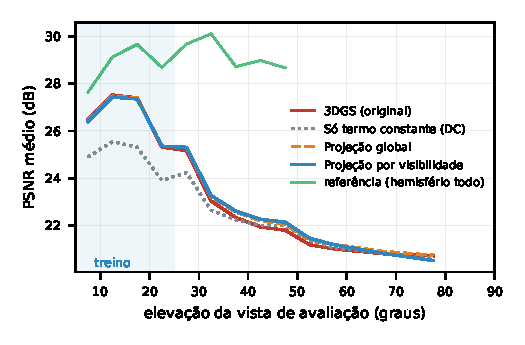
\includegraphics[width=\columnwidth]{figs/curva_elevacao_b25.pdf}
\caption{PSNR médio das seis cenas por elevação da vista de avaliação (intervalos de 5°), com treino só abaixo de 25° (área azul). Todas as variantes saem do mesmo modelo treinado; a linha verde é o modelo de referência, treinado com o hemisfério todo.}
\label{fig:curva}
\end{figure}

\subsection{QP2: oráculos mostram que cor e geometria se compensam}

\begin{table}[t]
\centering
\caption{PSNR (dB) fora da faixa de treino ($<25$°), nas vistas de índice ímpar de cada grupo. Oráculo: só a cor (SH) reajustada nas vistas de índice par do mesmo grupo, geometria congelada; é o teto de uma correção só de cor. Ref-G.: Ref-Gaussian treinado com as mesmas vistas.}
\label{tab:decomp25}
\setlength{\tabcolsep}{3pt}
\footnotesize
\begin{tabular}{l cccc cccc}
\toprule
 & \multicolumn{4}{c}{Acima} & \multicolumn{4}{c}{De cima} \\
\cmidrule(lr){2-5}\cmidrule(lr){6-9}
Cena & 3DGS & proj. & Ref-G. & oráculo & 3DGS & proj. & Ref-G. & oráculo \\
\midrule
\textit{ball} & 15{,}62 & 15{,}66 & 17{,}35 & 24{,}11 & 15{,}02 & 14{,}90 & 16{,}19 & 18{,}96 \\
\textit{car} & 21{,}68 & 21{,}72 & 22{,}93 & 27{,}24 & 19{,}64 & 19{,}48 & 20{,}92 & 26{,}05 \\
\textit{coffee} & 24{,}33 & 24{,}57 & 23{,}77 & 30{,}52 & 19{,}38 & 19{,}32 & 19{,}08 & 27{,}08 \\
\textit{helmet} & 22{,}33 & 22{,}61 & 22{,}65 & 28{,}89 & 21{,}29 & 21{,}45 & 20{,}75 & 27{,}08 \\
\textit{teapot} & 38{,}19 & 39{,}20 & 38{,}21 & 43{,}08 & 35{,}61 & 36{,}25 & 34{,}50 & 43{,}02 \\
\textit{toaster} & 13{,}90 & 13{,}98 & 17{,}33 & 20{,}06 & 14{,}86 & 14{,}90 & 16{,}19 & 20{,}14 \\
\midrule
Média & 22{,}68 & 22{,}96 & 23{,}71 & 28{,}98 & 20{,}97 & 21{,}05 & 21{,}27 & 27{,}05 \\
\bottomrule
\end{tabular}
\end{table}


O oráculo de cor, que reajusta todos os SH com a geometria congelada, eleva o PSNR de 21,0 para 27,1~dB de cima e de 22,7 para 29,0~dB acima (Tabela~\ref{tab:decomp25}), o nível da faixa filmada; a projeção fica longe desse teto. A Fig.~\ref{fig:qualitativo} mostra o efeito: mesmo com a cor ajustada apenas em vistas do lado oposto do objeto, a vista de 89° perde as manchas do 3DGS.

Os controles mudam a interpretação desse resultado (Tabela~\ref{tab:oraculos25}). Reajustar apenas a geometria, com a cor congelada, recupera ainda mais: 8,0~dB de cima. Reajustar apenas a cor constante recupera 4,1~dB. No controle mais rigoroso, com ajuste num lado do objeto e avaliação no outro, os ganhos caem para 2,3~dB (cor) e 3,1~dB (geometria), mas permanecem positivos. Cor e geometria, portanto, se substituem: a informação contida nas vistas de cima corrige a imagem por qualquer um dos dois caminhos. O modelo tem capacidade para representar a imagem correta; falta a informação.

\begin{table}[t]
\centering
\caption{Oráculos nas vistas de cima (PSNR em dB, treino abaixo de 25°). Cada oráculo reajusta só uma parte do modelo usando vistas de referência de cima: a cor constante de cada Gaussiana (DC), todos os SH (cor) ou posições, escalas, rotações e opacidades (geom.). Ímpares: ajuste nas vistas de índice par, avaliação nas ímpares. Lado oposto: ajuste num lado do objeto, avaliação no outro.}
\label{tab:oraculos25}
\setlength{\tabcolsep}{3pt}
\footnotesize
\begin{tabular}{l cccc ccc}
\toprule
 & \multicolumn{4}{c}{Ímpares} & \multicolumn{3}{c}{Lado oposto} \\
\cmidrule(lr){2-5}\cmidrule(lr){6-8}
Cena & 3DGS & DC & cor & geom. & 3DGS & cor & geom. \\
\midrule
\textit{ball} & 15{,}02 & 17{,}81 & 18{,}96 & 21{,}57 & 15{,}44 & 15{,}81 & 15{,}81 \\
\textit{car} & 19{,}64 & 23{,}87 & 26{,}05 & 27{,}22 & 19{,}56 & 22{,}90 & 23{,}79 \\
\textit{coffee} & 19{,}38 & 24{,}63 & 27{,}08 & 28{,}94 & 19{,}49 & 22{,}80 & 25{,}26 \\
\textit{helmet} & 21{,}29 & 24{,}50 & 27{,}08 & 27{,}74 & 21{,}37 & 22{,}50 & 23{,}03 \\
\textit{teapot} & 35{,}61 & 41{,}20 & 43{,}02 & 45{,}59 & 35{,}37 & 39{,}00 & 39{,}20 \\
\textit{toaster} & 14{,}86 & 18{,}31 & 20{,}14 & 22{,}49 & 15{,}04 & 17{,}08 & 17{,}51 \\
\midrule
Média & 20{,}97 & 25{,}06 & 27{,}05 & 28{,}92 & 21{,}04 & 23{,}35 & 24{,}10 \\
\bottomrule
\end{tabular}
\end{table}


\subsection{QP2: a geometria não piora de cima, mas está errada em todas as alturas}\label{sec:geometria}

O Shiny Blender fornece, para cada vista, a silhueta e o mapa de normais de referência, o que permite medir a geometria sem passar pela cor. Para cada vista de avaliação, renderizamos a opacidade acumulada e a profundidade esperada do modelo, derivamos as normais da profundidade (com suavização de 9~px) e as comparamos com a referência. Aplicado à profundidade de referência do conjunto, o mesmo cálculo erra entre 10° e 20°, limite imposto pela quantização da disparidade fornecida.

A Tabela~\ref{tab:geometria25} resume o resultado. A silhueta tem o mesmo IoU nos três grupos (0,91, 0,90 e 0,91). O erro das normais é alto em todos eles, de 54° a 63° em média: em objetos reflexivos, o 3DGS tende a imitar o reflexo com Gaussianas fora da superfície, e a profundidade resulta irregular. Esse erro é \emph{menor} de cima (53,8°) do que na faixa filmada (63,4°), provavelmente porque de cima predominam superfícies planas voltadas para a câmera. Uma segunda estimativa, sem suavização, confirma o quadro: tomando como normal o eixo mais curto de cada Gaussiana, composto por alfa, como no GaussianShader~\cite{jiang2024gshader}, o erro é de 55° na faixa, 48° acima e 41° de cima (Tabela~\ref{tab:normais25}).

\begin{table}[t]
\centering
\caption{Geometria medida contra a referência do Shiny Blender, treino abaixo de 25°: IoU da silhueta e erro angular médio (graus) das normais derivadas da profundidade renderizada. F: dentro da faixa; A: acima; C: de cima.}
\label{tab:geometria25}
\setlength{\tabcolsep}{4pt}
\footnotesize
\begin{tabular}{l ccc ccc}
\toprule
 & \multicolumn{3}{c}{IoU da silhueta$\uparrow$} & \multicolumn{3}{c}{Erro da normal (°)$\downarrow$} \\
\cmidrule(lr){2-4}\cmidrule(lr){5-7}
Cena & F & A & C & F & A & C \\
\midrule
\textit{ball} & 0{,}903 & 0{,}877 & 0{,}901 & 58{,}1 & 58{,}1 & 52{,}8 \\
\textit{car} & 0{,}925 & 0{,}957 & 0{,}967 & 63{,}2 & 59{,}7 & 55{,}7 \\
\textit{coffee} & 0{,}936 & 0{,}958 & 0{,}958 & 58{,}4 & 54{,}4 & 51{,}3 \\
\textit{helmet} & 0{,}957 & 0{,}953 & 0{,}961 & 66{,}9 & 62{,}1 & 53{,}7 \\
\textit{teapot} & 0{,}992 & 0{,}994 & 0{,}993 & 58{,}9 & 54{,}4 & 48{,}9 \\
\textit{toaster} & 0{,}741 & 0{,}665 & 0{,}674 & 74{,}9 & 69{,}0 & 60{,}6 \\
\midrule
Média & 0{,}909 & 0{,}901 & 0{,}909 & 63{,}4 & 59{,}6 & 53{,}8 \\
Treino completo$^\dagger$ & 0{,}939 & 0{,}965 & 0{,}984 & 58{,}3 & 57{,}0 & 52{,}5 \\
\bottomrule
\end{tabular}
\vspace{2pt}
{\scriptsize $^\dagger$ modelo treinado com as 100 vistas do hemisfério, média de 6 cenas (as vistas de cima fazem parte do treino dele).}
\end{table}


O modelo de referência separa duas componentes da geometria. Com vistas de cima no treino, a silhueta melhora (IoU de cima de 0,91 para 0,98) e a imagem também (+6,5~dB acima da faixa). A orientação da superfície, porém, praticamente não muda: o erro das normais de cima fica em 52,5°, contra 53,8° do modelo da faixa, embora essas vistas façam parte do treino dele. Um 3DGS que reproduz corretamente a imagem de cima também tem a superfície errada; no 3DGS, uma imagem correta não exige normal correta.

Junto com os oráculos, isso descreve o mecanismo. Em objetos reflexivos, o 3DGS não recupera a superfície em nenhuma altura, nem quando treinado com todas. Ele reproduz as vistas filmadas com uma geometria errada e uma cor dependente de vista que a compensa, e essa combinação só foi ajustada para as direções filmadas. De cima, a geometria não piora, mas a compensação deixa de valer.

\subsection{QP3: modelar a reflexão corrige a forma, não a aparência de cima}\label{sec:refgs}

O Ref-Gaussian~\cite{yao2025refgaussian} calcula o reflexo a partir da normal da superfície e de um único mapa de ambiente para a cena. Em princípio, isso permitiria reaproveitar o ambiente visto refletido numa parte do objeto para prever o reflexo de outra parte, vista de outro ângulo.

A geometria do Ref-Gaussian é de fato correta. Treinado com o hemisfério todo, ele erra as normais em 5,7° na faixa e 5,2° acima, na média das seis cenas, contra 41° a 63° do 3DGS conforme a estimativa e o grupo (Tabela~\ref{tab:normais25}). Treinado apenas na faixa, mantém a superfície correta também de cima: 11,6° de erro, contra 56,7° (profundidade) e 43,2° (eixo) do 3DGS nas mesmas três cenas.

\begin{table}[t]
\centering
\caption{Erro angular médio das normais (graus) contra a referência. No 3DGS, a normal é derivada da profundidade renderizada (prof.) ou é o eixo mais curto de cada Gaussiana, composto por alfa (eixo); no Ref-Gaussian, é a normal que o próprio modelo usa no sombreamento. Cada bloco usa só as cenas em que todos os seus modelos existem.}
\label{tab:normais25}
\setlength{\tabcolsep}{5pt}
\footnotesize
\begin{tabular}{l ccc}
\toprule
Modelo & Faixa & Acima & De cima \\
\midrule
\multicolumn{4}{l}{\textit{6 cenas}} \\
3DGS, faixa 25° (prof.) & 63{,}4 & 59{,}6 & 53{,}8 \\
3DGS, faixa 25° (eixo) & 54{,}5 & 48{,}0 & 40{,}8 \\
3DGS, hemisfério todo$^\dagger$ (prof.) & 58{,}3 & 57{,}0 & 52{,}5 \\
3DGS, hemisfério todo$^\dagger$ (eixo) & 54{,}9 & 49{,}9 & 43{,}4 \\
Ref-Gaussian, hemisfério todo & 5{,}7 & 5{,}2 & n/a \\
\midrule
\multicolumn{4}{l}{\textit{6 cenas}} \\
3DGS, faixa 25° (prof.) & 63{,}4 & 59{,}6 & 53{,}8 \\
3DGS, faixa 25° (eixo) & 54{,}5 & 48{,}0 & 40{,}8 \\
Ref-Gaussian, faixa 25° & 11{,}0 & 11{,}6 & 11{,}0 \\
\bottomrule
\end{tabular}
\vspace{2pt}
{\scriptsize $^\dagger$ as vistas de cima fazem parte do treino deste modelo.}
\end{table}


\textbf{Imagem.} Treinado só na faixa, o Ref-Gaussian melhora a imagem em todas as alturas, mas a vantagem diminui com a elevação: +2,1~dB na faixa (24,5 contra 22,3~dB nas mesmas três cenas), +1,7~dB acima e +0,7~dB de cima (19,3 contra 18,6~dB). No \textit{helmet}, fica abaixo do 3DGS de cima (20,6 contra 21,2~dB). Da faixa para cima, o Ref-Gaussian perde 5,2~dB e o 3DGS, 3,7~dB. A comparação é equilibrada em treino: o Ref-Gaussian da faixa usa 28 mil iterações, e o 3DGS, 30 mil. A Fig.~\ref{fig:qualitativo} mostra que, de cima, o Ref-Gaussian não apresenta os riscos brancos do 3DGS, mas a pintura e o metal saem borrados.

\textbf{A informação existe, e não são as iterações.} Treinado com o hemisfério todo, o mesmo método atinge, acima da faixa, 30,8~dB nessas três cenas, contra 21,0~dB do treinado só na faixa. O modelo completo usa o cronograma original de 50 mil iterações, e por isso avaliamos também seus \textit{checkpoints} intermediários (Tabela~\ref{tab:refgsiter25}). Com 30 mil iterações, ele já atinge 31,1~dB acima da faixa nessas cenas, e na média das seis cenas a diferença entre 30 e 50 mil iterações é de 0,05~dB (de $-$0,9 a +0,5~dB por cena; no \textit{helmet} e no \textit{toaster}, 30 mil é melhor). A distância de cerca de 10~dB entre o modelo da faixa e o completo vem, portanto, das vistas de cima, e não do treino mais longo.

\begin{table}[t]
\centering
\caption{Ref-Gaussian nas vistas de teste acima de 25° (PSNR em dB): treinado só na faixa, com 28 mil iterações, contra o modelo treinado com todas as alturas avaliado nos \textit{checkpoints} de 30, 40 e 50 mil iterações. A diferença entre as colunas do modelo completo mede o efeito das iterações; a diferença para a primeira coluna, o efeito das vistas de cima.}
\label{tab:refgsiter25}
\setlength{\tabcolsep}{4pt}
\footnotesize
\begin{tabular}{l c ccc}
\toprule
 & Faixa & \multicolumn{3}{c}{Todas as alturas} \\
\cmidrule(lr){2-2}\cmidrule(lr){3-5}
Cena & 28 mil & 30 mil & 40 mil & 50 mil \\
\midrule
\textit{ball} & -- & 35{,}46 & 35{,}66 & 35{,}92 \\
\textit{car} & 22{,}90 & 31{,}60 & 31{,}91 & 32{,}07 \\
\textit{coffee} & -- & 33{,}81 & 33{,}97 & 34{,}10 \\
\textit{helmet} & 22{,}63 & 33{,}32 & 34{,}01 & 32{,}41 \\
\textit{teapot} & -- & 48{,}42 & 48{,}47 & 48{,}56 \\
\textit{toaster} & 17{,}30 & 28{,}25 & 28{,}68 & 28{,}05 \\
\midrule
Média (3 cenas) & 20{,}95 & 31{,}05 & 31{,}53 & 30{,}84 \\
\bottomrule
\end{tabular}
\end{table}


\textbf{O ambiente refletido de cima já foi observado.} Para cada pixel do objeto, calculamos a direção refletida com a normal de referência e marcamos, numa grade da esfera com células de 5°, as direções que aparecem nas vistas de treino. Em todas as seis cenas, 100\% das direções refletidas nas vistas de cima já aparecem em alguma vista de treino; no \textit{car}, no \textit{helmet} e no \textit{ball}, com a mesma densidade das vistas da faixa. Superfícies curvas refletem quase a esfera inteira de qualquer ponto de vista. Para um modelo com mapa de ambiente compartilhado, a informação sobre a iluminação de cima está disponível.

\textbf{O que falta: oráculos por componente.} Para identificar a parte da aparência que falha, aplicamos ao Ref-Gaussian o mesmo protocolo de oráculos do 3DGS: com a geometria congelada, reajustamos com as vistas de cima de índice par apenas o material (cor base, cor difusa, intensidade do reflexo, rugosidade e metalicidade de cada Gaussiana), apenas o mapa de ambiente, apenas a luz indireta aprendida, ou as três partes, e avaliamos nas vistas de índice ímpar (1000 passos de Adam com as taxas do treino). A Tabela~\ref{tab:refgsoraculos25} resume o resultado. O material é a componente que mais recupera: +1,6~dB em média, contra +0,6~dB do mapa de ambiente e +0,2~dB da luz indireta. Isso concorda com o teste de cobertura: o ambiente foi observado; o que não foi observado é como cada superfície voltada para cima reflete. Com câmeras abaixo de 25°, uma superfície horizontal só é vista a mais de 65° da sua normal, e sua rugosidade e intensidade de reflexo são ajustadas apenas nesses ângulos rasantes.

\begin{table*}[t]
\centering
\caption{Oráculos de cima, treino abaixo de 25° (PSNR em dB nas vistas de cima de índice ímpar; o ajuste usa as de índice par). No 3DGS, reajusta-se só a cor (SH) ou só a geometria. No Ref-Gaussian, reajusta-se só o material (cor base, cor difusa, intensidade do reflexo, rugosidade, metalicidade), só o mapa de ambiente, só a luz indireta, as três (aparência), só a geometria (posições, formas, opacidades e normais) ou tudo. No \textit{ball} há apenas cinco vistas de avaliação.}
\label{tab:refgsoraculos25}
\setlength{\tabcolsep}{4pt}
\footnotesize
\begin{tabular}{l ccc ccccccc}
\toprule
 & \multicolumn{3}{c}{3DGS} & \multicolumn{7}{c}{Ref-Gaussian} \\
\cmidrule(lr){2-4}\cmidrule(lr){5-11}
Cena & orig. & cor & geom. & orig. & material & ambiente & indireta & aparência & geometria & tudo \\
\midrule
\textit{ball} & 15{,}02 & 18{,}96 & 21{,}57 & 16{,}19 & 18{,}70 & 16{,}75 & 16{,}20 & 20{,}22 & 21{,}00 & 23{,}32 \\
\textit{car} & 19{,}64 & 26{,}05 & 27{,}22 & 20{,}92 & 23{,}08 & 21{,}71 & 20{,}94 & 23{,}73 & 26{,}94 & 27{,}87 \\
\textit{coffee} & 19{,}38 & 27{,}08 & 28{,}94 & 19{,}08 & 23{,}22 & 19{,}30 & 19{,}17 & 23{,}56 & 27{,}45 & 27{,}87 \\
\textit{helmet} & 21{,}29 & 27{,}08 & 27{,}74 & 20{,}75 & 22{,}08 & 21{,}40 & 21{,}17 & 23{,}58 & 27{,}28 & 28{,}21 \\
\textit{teapot} & 35{,}61 & 43{,}02 & 45{,}59 & 34{,}51 & 35{,}14 & 35{,}27 & 34{,}62 & 37{,}48 & 41{,}37 & 42{,}34 \\
\textit{toaster} & 14{,}86 & 20{,}14 & 22{,}49 & 16{,}19 & 17{,}46 & 16{,}68 & 16{,}32 & 18{,}56 & 22{,}16 & 23{,}08 \\
\midrule
Média (6) & 20{,}97 & 27{,}05 & 28{,}92 & 21{,}27 & 23{,}28 & 21{,}85 & 21{,}40 & 24{,}52 & 27{,}70 & 28{,}78 \\
\bottomrule
\end{tabular}
\end{table*}


Mesmo reajustando toda a aparência, porém, o Ref-Gaussian recupera apenas 2,7~dB de cima, contra 5,8~dB do oráculo de cor do 3DGS. A aparência do Ref-Gaussian é restrita pela física: a cor é calculada a partir da normal e do mapa de ambiente, e não pode compensar livremente uma geometria imperfeita, como os SH do 3DGS fazem. A geometria residual pesa mais nesse caso, porque o reflexo amplifica o erro de orientação: num espelho, uma normal desviada de $\theta$ desvia a direção refletida de $2\theta$, e os 11,6° de erro de normal de cima podem deslocar o reflexo em mais de 20°. A restrição física que dá ao Ref-Gaussian uma geometria correta é a mesma que o impede de compensar, pela aparência, o que falta de cima.

\begin{figure*}[t]
\centering
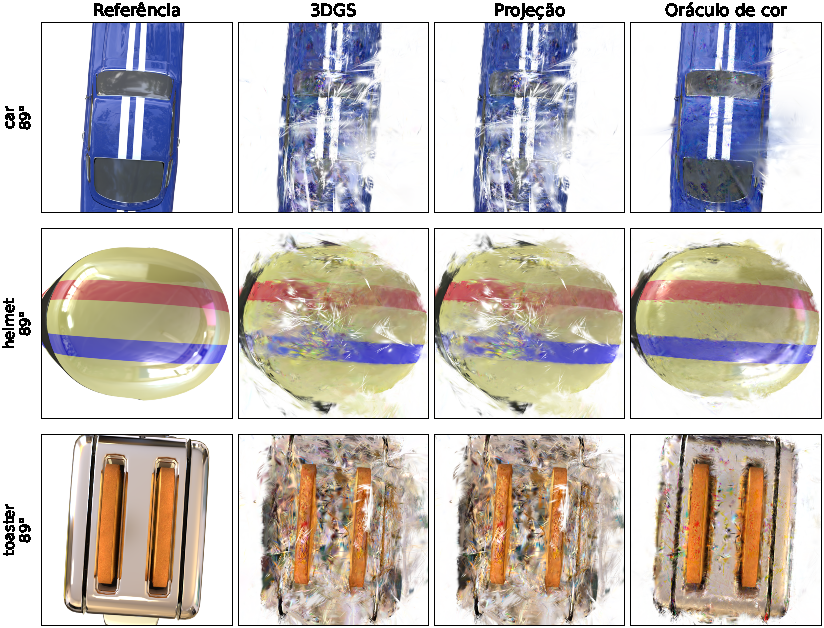
\includegraphics[width=0.8\textwidth]{figs/qualitativo_cima.pdf}
\caption{A vista mais alta de cada cena (89°), com treino só abaixo de 25°. A projeção remove pouco das manchas do 3DGS. No oráculo de cor, a geometria é a mesma e só a cor foi reajustada, em vistas de cima do lado oposto do objeto; esta vista não entrou no ajuste. O Ref-Gaussian, treinado nas mesmas vistas, tem a superfície correta, mas a aparência de cima continua borrada.}
\label{fig:qualitativo}
\end{figure*}

\subsection{QP4: a projeção é segura na faixa, mas recupera pouco}

\textbf{Dentro da faixa.} As duas projeções mudam o PSNR em menos de 0,1~dB (0,02~dB a global e 0,06~dB a por visibilidade), como prevê a garantia da Seção~\ref{sec:metodo}, e o LPIPS melhora ligeiramente. Descartar toda a dependência de vista (grau 0) custa 1,8~dB: os reflexos observados pelas câmeras são reais e precisam ser mantidos.

\textbf{Acima da faixa.} A projeção por visibilidade ganha 0,28~dB em média. O intervalo de confiança de 95\% por \textit{bootstrap} nas 642 vistas vai de 0,25 a 0,31~dB, e 84\% das vistas melhoram. Esse é o efeito previsto: as combinações de coeficientes que nenhuma câmera fixou são removidas, e com elas parte do reflexo inventado. O ganho, porém, é pequeno diante dos 4~dB perdidos e concentra-se numa cena: no \textit{teapot}, de cor quase uniforme, a projeção ganha 1,0~dB; nas outras cinco, entre 0,03 e 0,27~dB (Tabela~\ref{tab:cenas25}).

\begin{table}[t]
\centering
\caption{PSNR (dB) por cena, treino abaixo de 25°: 3DGS original e com a projeção por visibilidade ($\Delta$ = ganho).}
\label{tab:cenas25}
\setlength{\tabcolsep}{4pt}
\begin{tabular}{l ccc ccc}
\toprule
 & \multicolumn{3}{c}{Acima} & \multicolumn{3}{c}{De cima} \\
\cmidrule(lr){2-4}\cmidrule(lr){5-7}
Cena & orig. & proj. & $\Delta$ & orig. & proj. & $\Delta$ \\
\midrule
\textit{ball} & 15{,}62 & 15{,}65 & +0{,}03 & 14{,}55 & 14{,}44 & -0{,}12 \\
\textit{car} & 21{,}66 & 21{,}71 & +0{,}05 & 19{,}70 & 19{,}52 & -0{,}18 \\
\textit{coffee} & 24{,}31 & 24{,}55 & +0{,}24 & 19{,}51 & 19{,}45 & -0{,}05 \\
\textit{helmet} & 22{,}33 & 22{,}60 & +0{,}27 & 21{,}20 & 21{,}35 & +0{,}14 \\
\textit{teapot} & 38{,}19 & 39{,}20 & +1{,}01 & 35{,}64 & 36{,}32 & +0{,}67 \\
\textit{toaster} & 13{,}92 & 14{,}00 & +0{,}08 & 14{,}80 & 14{,}81 & +0{,}00 \\
\bottomrule
\end{tabular}
\end{table}


\textbf{De cima.} Nenhuma variante funciona. A projeção ganha 0,08~dB na média das cenas, apenas 48\% das vistas melhoram e em três cenas o PSNR piora. O grau 0 é o resultado mais revelador: sem nenhuma dependência de vista, o modelo atinge 20,93~dB de cima, o mesmo que o original (20,90~dB). Vistos de cima, os 15 coeficientes direcionais aprendidos valem tanto quanto a ausência de reflexo. A Tabela~\ref{tab:lambda} mostra que o resultado não depende de $\lambda$: com $10^{-3}$ a projeção quase não atua, e com $10^{-1}$ custa 0,3~dB na faixa sem ganhar de cima.

\begin{table}[t]
\centering
\caption{Sensibilidade à regularização $\lambda$ (PSNR médio em dB, faixa de 25°).}
\label{tab:lambda}
\begin{tabular}{l ccc}
\toprule
Projeção & Faixa & Acima & De cima \\
\midrule
sem projeção (original) & 26{,}73 & 22{,}67 & 20{,}90 \\
global, $\lambda=10^{-2}$ & 26{,}71 & 22{,}89 & 21{,}03 \\
visibilidade, $\lambda=10^{-3}$ & 26{,}71 & 22{,}79 & 20{,}85 \\
visibilidade, $\lambda=10^{-2}$ & 26{,}67 & 22{,}95 & 20{,}98 \\
visibilidade, $\lambda=10^{-1}$ & 26{,}44 & 22{,}96 & 21{,}00 \\
\bottomrule
\end{tabular}
\end{table}


Com a faixa de 15°, a projeção global continua neutra na faixa (22,68 contra 22,69~dB), mas a projeção por visibilidade passa a piorá-la em 0,25~dB (IC~95\%: 0,20 a 0,29~dB) e não ganha fora dela ($-$0,02~dB acima e $-$0,13~dB de cima). Com cerca de 17 câmeras, as vistas de teste da faixa ficam entre as direções de treino, onde a garantia não vale, e a versão por visibilidade, que usa só as câmeras que veem cada Gaussiana, é mais agressiva justamente onde há menos câmeras.

\subsection{QP4: custo e qualidade das correções leves}

\begin{table*}[t]
\centering
\caption{Correções aplicadas ao modelo já treinado (treino abaixo de 25°), sem retreino: tempo na GPU, tamanho médio do modelo em precisão simples e qualidade por grupo, média de 6 cenas. Em negrito, o melhor de cada coluna de qualidade. Para comparação, o retreino com vistas de cima chega a 28,6 e 29,1~dB na faixa e acima, e o Ref-Gaussian exige um novo treino cerca de 1,9 vez mais longo que o do 3DGS.}
\label{tab:custo25}
\setlength{\tabcolsep}{4pt}
\begin{tabular}{l cc ccc c}
\toprule
 & \multicolumn{2}{c}{Custo} & \multicolumn{3}{c}{PSNR (dB)$\uparrow$} & LPIPS$\downarrow$ \\
\cmidrule(lr){2-3}\cmidrule(lr){4-6}\cmidrule(lr){7-7}
Correção & Tempo (s) & Tamanho (MB) & Faixa & Acima & De cima & De cima \\
\midrule
3DGS original (grau 3) & -- & 61{,}6 & \textbf{26{,}73} & 22{,}67 & 20{,}90 & 0{,}256 \\
\midrule
Truncamento, grau 0 & 0{,}13 & 14{,}6 & 24{,}98 & 22{,}53 & 20{,}93 & \textbf{0{,}246} \\
Truncamento, grau 1 & 0{,}07 & 24{,}0 & 25{,}63 & \textbf{23{,}03} & \textbf{21{,}28} & 0{,}247 \\
Truncamento, grau 2 & 0{,}06 & 39{,}7 & 26{,}19 & 23{,}02 & 21{,}18 & 0{,}248 \\
Grau adaptativo~\cite{papantonakis2024reducing} & 1{,}16 & 54{,}5 & 26{,}73 & 22{,}67 & 20{,}90 & 0{,}255 \\
Projeção global & 0{,}07 & 61{,}6 & 26{,}71 & 22{,}89 & 21{,}03 & 0{,}249 \\
Projeção global + grau adapt. & 0{,}19 & 57{,}8 & 26{,}70 & 22{,}90 & 21{,}04 & 0{,}249 \\
Projeção por visibilidade & 1{,}19 & 61{,}6 & 26{,}67 & 22{,}95 & 20{,}98 & 0{,}247 \\
Projeção por visib. + grau adapt. & 1{,}30 & 53{,}1 & 26{,}65 & 22{,}95 & 20{,}98 & 0{,}247 \\
\bottomrule
\end{tabular}
\end{table*}


A Tabela~\ref{tab:custo25} e a Fig.~\ref{fig:custo} comparam as correções aplicadas ao modelo já treinado. Elas formam um compromisso entre preservar a faixa filmada e melhorar o que está fora dela. O truncamento para grau 1 ou 2 é o que mais melhora as vistas fora da faixa (+0,36 e +0,35~dB acima; +0,38 e +0,28~dB de cima) e reduz o modelo de 61,6 para 24,0 e 39,7~MB, mas custa 1,1 e 0,5~dB dentro da faixa. A projeção não custa nada na faixa ($-$0,02~dB a global e $-$0,06~dB a por visibilidade) e ganha de 0,22 a 0,28~dB acima dela, mas só de 0,08 a 0,13~dB de cima, sem reduzir o tamanho. O grau adaptativo, com a tolerância usada, preserva a qualidade e reduz o modelo em 12\% (54,5~MB); depois da projeção por visibilidade, a redução chega a 14\% (53,1~MB), porque a projeção atenua parte dos termos não observados. Todas as correções custam de centésimos de segundo a pouco mais de 1~s na GPU, e a projeção global, a única que dispensa câmeras e GPU, roda em 0,6~s em CPU no veículo real de 273 mil Gaussianas. Nenhuma correção leve recupera mais de 0,4~dB dos 5,8~dB perdidos de cima.

\begin{figure}[t]
\centering
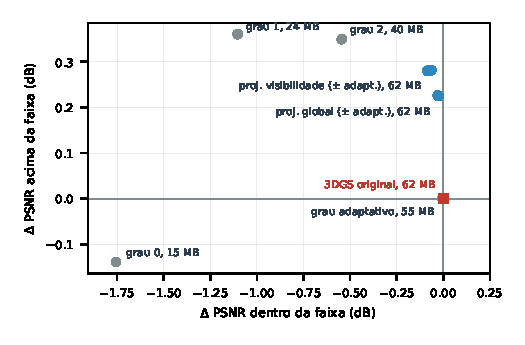
\includegraphics[width=\columnwidth]{figs/custo_qualidade_b25.pdf}
\caption{Compromisso das correções sem retreino, média das seis cenas: variação de PSNR dentro da faixa filmada (eixo horizontal) contra variação acima dela (eixo vertical), em relação ao 3DGS original. O rótulo traz o tamanho do modelo. As projeções preservam a faixa; o truncamento ganha um pouco mais fora dela, ao custo da faixa.}
\label{fig:custo}
\end{figure}

\subsection{Veículo real}

No Porsche 911 (273 mil Gaussianas, câmeras entre 0,4° e 3,8°), não há referência de cima. Medimos então quanto a projeção global altera a imagem, comparando as renderizações antes e depois dela numa volta completa em cada elevação. Na faixa filmada (2°), o PSNR entre as duas é de 49,6~dB: a mudança é imperceptível, como prevê a garantia. Acima, cai para 37,8~dB a 20°, 35,1~dB a 45° e 39,0~dB a 89°. A mudança existe, mas é pequena, e a Fig.~\ref{fig:teaser} mostra que ela não remove as manchas do teto e do capô. O comportamento é o mesmo do laboratório sintético. A ferramenta de linha de comando aplica essa projeção ao arquivo \texttt{.ply} do veículo em 0,6~s, em CPU.

% =====================================================================
\section{Discussão}\label{sec:discussao}

\textbf{Respostas às questões de pesquisa.} (QP1) A perda fora da faixa filmada é grande, 5,8~dB de cima com a faixa de 25° e 10,2~dB acima da faixa com a de 15°, e decorre da cobertura, não da dificuldade das vistas. (QP2) Ela não vem de uma geometria que piora onde nenhuma câmera olhou: silhueta e normais vistas de cima não são piores que na faixa. Em objetos reflexivos, o 3DGS reproduz as vistas filmadas com uma superfície errada e uma cor que a compensa; de cima, essa compensação deixa de valer, e reajustar com vistas de cima tanto a cor quanto a forma devolve a qualidade. (QP3) O Ref-Gaussian corrige a forma (11,6° de erro de normal de cima, contra 56,7° do 3DGS) e melhora a imagem, mas a vantagem cai de 2,1~dB na faixa para 0,7~dB de cima. O ambiente refletido de cima já havia sido observado; dentro da aparência, o que mais falta é o material das superfícies voltadas para cima, e a restrição física impede que a aparência compense o erro de geometria que resta, amplificado pelo reflexo. Com as vistas de cima, o mesmo método ganha cerca de 10~dB acima da faixa, e as iterações a mais não explicam esse ganho. (QP4) Correções aplicadas ao modelo treinado, sem informação nova, recuperam no máximo 0,4~dB. A pergunta ``cor ou geometria?'' pressupõe que as duas sejam separáveis; no 3DGS, em superfícies reflexivas, não são, e a mesma imagem filmada admite muitas combinações de forma e cor.

\textbf{Quando usar cada correção.} Os resultados indicam uma escolha por cenário. \textit{(a) Visualização de anúncios na web ou em celular}, com orçamento de memória e de banda. Quando o comprador olha sobretudo ao redor do veículo, a projeção global é a escolha: não altera a faixa filmada, reduz os reflexos inventados logo acima dela, roda em CPU sobre o arquivo final e pode ser seguida do grau adaptativo para economizar memória. Quando o tamanho pesa mais e o visualizador permite órbita livre, o truncamento para grau 2 troca 0,5~dB na faixa por 0,35~dB acima dela e 36\% de memória a menos (Tabela~\ref{tab:custo25}). Em ambos os casos, a câmera do visualizador deve ficar limitada à faixa coberta, já que nenhuma correção leve recupera a vista de topo. \textit{(b) Inspeção de veículos}, em que inventar detalhes é inaceitável: correções gerativas~\cite{wu2025difix3d,liu2024viewextrapolator} não são adequadas, e o caminho é sinalizar as vistas extrapoladas ou capturar a altura que falta; a matriz de Gram fornece essa sinalização por Gaussiana. \textit{(c) Simulação a partir de gravações de direção}, que precisa de vistas distantes da trajetória: correções leves são insuficientes, e a informação precisa vir de priors gerativos~\cite{wang2025freevs} ou de gravações com múltiplas passagens~\cite{han2025euvs}. Em todos os casos, um modelo físico como o Ref-Gaussian melhora a geometria e a imagem dentro e perto da faixa, ao custo de um treino cerca de 2,4 vezes mais longo (47 contra 20~min por cena na mesma GPU), e é a base mais promissora para incorporar conhecimento prévio sobre materiais.

\textbf{Extensão para cenas 4D automotivas.} O problema estudado aqui é mais severo em cenas dinâmicas de direção. As câmeras são fixas no veículo, cada instante é observado de um único conjunto de alturas, e os agentes em movimento são vistos de ângulos ainda mais restritos. Três elementos deste trabalho se estendem diretamente a esse caso. Primeiro, a análise de condicionamento: representações dinâmicas baseadas em Gaussianas mantêm cor por SH, inclusive variável no tempo~\cite{yan2024streetgs,wu2024gs4d}, e a matriz de Gram de cada Gaussiana pode ser calculada por janela de tempo, com os mesmos pesos de visibilidade obtidos pelo rasterizador. Segundo, o protocolo: simuladores como o CARLA~\cite{dosovitskiy2017carla} fornecem referência exata de qualquer altura, o que permite repetir o controle de cobertura e os oráculos em cenas dinâmicas, enquanto conjuntos reais com múltiplas passagens~\cite{han2025euvs} validam o resultado. Terceiro, a decomposição por oráculos, que em 4D separaria aparência, forma e movimento. Representações com primitivas explícitas são a base natural para essa extensão, porque cada Gaussiana tem posição, movimento e cor próprios, o que permite os diagnósticos por primitiva usados aqui, difíceis de aplicar a representações implícitas.

\textbf{Limitações.} (i) Os oráculos usam as vistas de referência de cima e medem um teto, não um método; como cor e forma se substituem, nenhum isola uma causa sozinho, e a conclusão decorre da combinação deles com a medida direta da geometria. (ii) O 3DGS não tem normal própria; as duas estimativas usadas (profundidade e eixo mais curto) concordam, mas são aproximações. (iii) As métricas de imagem são calculadas na imagem inteira com fundo branco, o que soma o fundo, fácil, às médias. (iv) As cenas sintéticas têm materiais muito reflexivos; veículos reais combinam pintura, vidro e plástico. (v) Cada configuração foi treinada com uma única semente; os intervalos de confiança refletem a variação entre vistas, não entre treinos. (vi) Por custo de GPU, o Ref-Gaussian foi treinado na faixa em três cenas e com 28 mil iterações; o controle com os \textit{checkpoints} do modelo completo indica que as iterações pesam pouco, mas o cronograma escalado não é idêntico ao original. (vii) A garantia da projeção vale nas direções de treino; com a faixa de 15°, a versão por visibilidade piora as vistas de teste da própria faixa, e só a global permanece neutra. (viii) Os oráculos do Ref-Gaussian usam 1000 passos, contra 3000 nos do 3DGS, e mantêm a malha usada na luz indireta; seus ganhos são, portanto, limites inferiores do que cada componente poderia recuperar.

\textbf{Trabalhos futuros.} (i) Completar a decomposição do Ref-Gaussian com um oráculo de geometria (posições, formas e normais), que mediria quanto do erro de cima vem do desvio residual das normais amplificado pelo reflexo. (ii) Aprender um prior de materiais com objetos sintéticos observados de todos os ângulos e usá-lo dentro do Ref-Gaussian, que já tem geometria e ambiente corretos e onde o material é a componente que mais falta. (iii) Repetir o protocolo em cenas dinâmicas de direção, com o CARLA e com conjuntos reais de múltiplas passagens. (iv) Comparar, no mesmo protocolo, correções gerativas como Difix3D+~\cite{wu2025difix3d}, medindo também quanto elas inventam. (v) Usar a matriz de Gram como mapa de confiança por Gaussiana, para guiar a captura e sinalizar vistas extrapoladas. (vi) Repetir os treinos com várias sementes e medir as métricas só nos pixels do objeto.

% =====================================================================
\section{Conclusão}\label{sec:conclusao}

Este trabalho mediu, num cenário controlado e com foco no domínio automotivo, o que acontece quando um modelo 3DGS treinado com vistas numa faixa estreita de elevação é visto de cima. A perda média é de 5,8~dB de PSNR com a faixa de 25° e cresce com faixas mais estreitas. A análise da matriz de Gram mostra que uma faixa estreita deixa a maior parte dos coeficientes de cor indeterminada, e uma projeção sem treino, com garantia de alterar pouco as direções observadas, remove esses coeficientes em menos de 1~s. Ela melhora as vistas logo acima da faixa (+0,28~dB, 84\% das vistas), mas quase nada de cima. Oráculos e a medida direta da geometria mostram o motivo: a geometria vista de cima não é pior que a da faixa, mas está errada em todas as alturas, e o modelo reproduz as vistas filmadas compensando-a com a cor. O Ref-Gaussian, modelo de reflexão baseado em física, corrige a forma (12° de erro de normal de cima, contra 57°), mas perde de cima tanto quanto o 3DGS, embora o ambiente refletido de cima já tivesse aparecido no treino. Oráculos por componente mostram que, na aparência dele, o que mais falta é o material das superfícies vistas só de raspão, e que a restrição física, que garante a forma correta, impede a aparência de compensar o erro de normal que resta. Com as vistas de cima, o mesmo método ganha cerca de 10~dB, e o controle por \textit{checkpoints} mostra que esse ganho não vem das iterações. Fora do ângulo filmado falta informação, não ajuste. Correções leves têm lugar em visualização com orçamento de memória, desde que acompanhadas da limitação do ponto de vista; vistas distantes exigem captura adicional ou conhecimento prévio. A extensão natural é o caso dinâmico das gravações de direção, em que a cobertura limitada é a regra.


% =====================================================================
\section*{Disponibilidade de código}
O código dos experimentos, os resultados por vista em JSON (dos quais todas as tabelas são geradas) e a ferramenta \texttt{projetar\_ply.py}, que aplica a projeção global a qualquer modelo 3DGS no formato \texttt{.ply}, estão em \url{https://github.com/Pimenta15/Gaussian-Splating}, na pasta \texttt{experimentos/extrapolacao\_sh}. Uma demonstração interativa, na pasta \texttt{documentacao/demo} do mesmo repositório, permite percorrer a elevação em cada cena e comparar lado a lado a referência, o 3DGS e o Ref-Gaussian treinados na faixa e com cobertura completa, e as correções leves.

\begin{thebibliography}{00}
\bibitem{kerbl2023} B. Kerbl, G. Kopanas, T. Leimkühler, and G. Drettakis, ``3D Gaussian splatting for real-time radiance field rendering,'' \textit{ACM Trans. Graph.}, vol. 42, no. 4, 2023, doi: \href{https://doi.org/10.1145/3592433}{10.1145/3592433}.
\bibitem{mildenhall2022nerf} B. Mildenhall, P. P. Srinivasan, M. Tancik, J. T. Barron, R. Ramamoorthi, and R. Ng, ``NeRF: Representing scenes as neural radiance fields for view synthesis,'' \textit{Commun. ACM}, vol. 65, no. 1, pp. 99--106, 2022, doi: \href{https://doi.org/10.1145/3503250}{10.1145/3503250}.
\bibitem{fei2024survey} B. Fei, J. Xu, R. Zhang, Q. Zhou, W. Yang, and Y. He, ``3D Gaussian splatting as a new era: A survey,'' \textit{IEEE Trans. Vis. Comput. Graph.}, 2024, doi: \href{https://doi.org/10.1109/TVCG.2024.3397828}{10.1109/TVCG.2024.3397828}.
\bibitem{verbin2022refnerf} D. Verbin, P. Hedman, B. Mildenhall, T. Zickler, J. T. Barron, and P. P. Srinivasan, ``Ref-NeRF: Structured view-dependent appearance for neural radiance fields,'' in \textit{Proc. IEEE/CVF Conf. Comput. Vis. Pattern Recognit. (CVPR)}, 2022. [Online]. Available: \url{https://arxiv.org/abs/2112.03907}
\bibitem{ramamoorthi2001irradiance} R. Ramamoorthi and P. Hanrahan, ``An efficient representation for irradiance environment maps,'' in \textit{Proc. ACM SIGGRAPH}, 2001, pp. 497--500, doi: \href{https://doi.org/10.1145/383259.383317}{10.1145/383259.383317}.
\bibitem{sloan2002prt} P.-P. Sloan, J. Kautz, and J. Snyder, ``Precomputed radiance transfer for real-time rendering in dynamic, low-frequency lighting environments,'' \textit{ACM Trans. Graph.}, vol. 21, no. 3, 2002, doi: \href{https://doi.org/10.1145/566654.566612}{10.1145/566654.566612}.
\bibitem{yu2021plenoctrees} A. Yu, R. Li, M. Tancik, H. Li, R. Ng, and A. Kanazawa, ``PlenOctrees for real-time rendering of neural radiance fields,'' in \textit{Proc. IEEE/CVF Int. Conf. Comput. Vis. (ICCV)}, 2021. [Online]. Available: \url{https://arxiv.org/abs/2103.14024}
\bibitem{fridovich2022plenoxels} S. Fridovich-Keil, A. Yu, M. Tancik, Q. Chen, B. Recht, and A. Kanazawa, ``Plenoxels: Radiance fields without neural networks,'' in \textit{Proc. IEEE/CVF Conf. Comput. Vis. Pattern Recognit. (CVPR)}, 2022. [Online]. Available: \url{https://arxiv.org/abs/2112.05131}
\bibitem{yang2024spec} Z. Yang, X. Gao, Y. Sun, Y. Huang, X. Lyu, W. Zhou, S. Jiao, X. Qi, and X. Jin, ``Spec-Gaussian: Anisotropic view-dependent appearance for 3D Gaussian splatting,'' in \textit{Adv. Neural Inf. Process. Syst. (NeurIPS)}, vol. 37, 2024. [Online]. Available: \url{https://arxiv.org/abs/2402.15870}
\bibitem{liu2023nero} Y. Liu, P. Wang, C. Lin, X. Long, J. Wang, L. Liu, T. Komura, and W. Wang, ``NeRO: Neural geometry and BRDF reconstruction of reflective objects from multiview images,'' \textit{ACM Trans. Graph.}, vol. 42, no. 4, 2023, doi: \href{https://doi.org/10.1145/3592134}{10.1145/3592134}.
\bibitem{verbin2024nerfcasting} D. Verbin, P. P. Srinivasan, P. Hedman, B. Mildenhall, B. Attal, R. Szeliski, and J. T. Barron, ``NeRF-Casting: Improved view-dependent appearance with consistent reflections,'' in \textit{Proc. ACM SIGGRAPH Asia}, 2024. [Online]. Available: \url{https://arxiv.org/abs/2405.14871}
\bibitem{jiang2024gshader} Y. Jiang, J. Tu, Y. Liu, X. Gao, X. Long, W. Wang, and Y. Ma, ``GaussianShader: 3D Gaussian splatting with shading functions for reflective surfaces,'' in \textit{Proc. IEEE/CVF Conf. Comput. Vis. Pattern Recognit. (CVPR)}, 2024, pp. 5322--5332. [Online]. Available: \url{https://arxiv.org/abs/2311.17977}
\bibitem{ye2024gsdr} K. Ye, Q. Hou, and K. Zhou, ``3D Gaussian splatting with deferred reflection,'' in \textit{Proc. ACM SIGGRAPH Conf. Papers}, 2024, doi: \href{https://doi.org/10.1145/3641519.3657456}{10.1145/3641519.3657456}.
\bibitem{huang2024gs2d} B. Huang, Z. Yu, A. Chen, A. Geiger, and S. Gao, ``2D Gaussian splatting for geometrically accurate radiance fields,'' in \textit{Proc. ACM SIGGRAPH Conf. Papers}, 2024, doi: \href{https://doi.org/10.1145/3641519.3657428}{10.1145/3641519.3657428}.
\bibitem{yao2025refgaussian} Y. Yao, Z. Zeng, C. Gu, X. Zhu, and L. Zhang, ``Reflective Gaussian splatting,'' in \textit{Proc. Int. Conf. Learn. Represent. (ICLR)}, 2025. [Online]. Available: \url{https://arxiv.org/abs/2412.19282}
\bibitem{fan2024lightgaussian} Z. Fan, K. Wang, K. Wen, Z. Zhu, D. Xu, and Z. Wang, ``LightGaussian: Unbounded 3D Gaussian compression with 15x reduction and 200+ FPS,'' in \textit{Adv. Neural Inf. Process. Syst. (NeurIPS)}, vol. 37, 2024. [Online]. Available: \url{https://arxiv.org/abs/2311.17245}
\bibitem{papantonakis2024reducing} P. Papantonakis, G. Kopanas, B. Kerbl, A. Lanvin, and G. Drettakis, ``Reducing the memory footprint of 3D Gaussian splatting,'' \textit{Proc. ACM Comput. Graph. Interact. Tech.}, vol. 7, no. 1, 2024, doi: \href{https://doi.org/10.1145/3651282}{10.1145/3651282}.
\bibitem{niemeyer2022regnerf} M. Niemeyer, J. T. Barron, B. Mildenhall, M. S. M. Sajjadi, A. Geiger, and N. Radwan, ``RegNeRF: Regularizing neural radiance fields for view synthesis from sparse inputs,'' in \textit{Proc. IEEE/CVF Conf. Comput. Vis. Pattern Recognit. (CVPR)}, 2022. [Online]. Available: \url{https://arxiv.org/abs/2112.00724}
\bibitem{yang2023freenerf} J. Yang, M. Pavone, and Y. Wang, ``FreeNeRF: Improving few-shot neural rendering with free frequency regularization,'' in \textit{Proc. IEEE/CVF Conf. Comput. Vis. Pattern Recognit. (CVPR)}, 2023. [Online]. Available: \url{https://arxiv.org/abs/2303.07418}
\bibitem{zhu2024fsgs} Z. Zhu, Z. Fan, Y. Jiang, and Z. Wang, ``FSGS: Real-time few-shot view synthesis using Gaussian splatting,'' in \textit{Proc. Eur. Conf. Comput. Vis. (ECCV)}, 2024, doi: \href{https://doi.org/10.1007/978-3-031-72933-1_9}{10.1007/978-3-031-72933-1\_9}.
\bibitem{li2024dngaussian} J. Li, J. Zhang, X. Bai, J. Zheng, X. Ning, J. Zhou, and L. Gu, ``DNGaussian: Optimizing sparse-view 3D Gaussian radiance fields with global-local depth normalization,'' in \textit{Proc. IEEE/CVF Conf. Comput. Vis. Pattern Recognit. (CVPR)}, 2024. [Online]. Available: \url{https://arxiv.org/abs/2403.06912}
\bibitem{wu2024reconfusion} R. Wu, B. Mildenhall, P. Henzler, K. Park, R. Gao, D. Watson, P. P. Srinivasan, D. Verbin, J. T. Barron, B. Poole, and A. Hołyński, ``ReconFusion: 3D reconstruction with diffusion priors,'' in \textit{Proc. IEEE/CVF Conf. Comput. Vis. Pattern Recognit. (CVPR)}, 2024. [Online]. Available: \url{https://arxiv.org/abs/2312.02981}
\bibitem{gao2024cat3d} R. Gao, A. Hołyński, P. Henzler, A. Brussee, R. Martin-Brualla, P. Srinivasan, J. T. Barron, and B. Poole, ``CAT3D: Create anything in 3D with multi-view diffusion models,'' in \textit{Adv. Neural Inf. Process. Syst. (NeurIPS)}, vol. 37, 2024. [Online]. Available: \url{https://arxiv.org/abs/2405.10314}
\bibitem{yang2024gaussianobject} C. Yang, S. Li, J. Fang, R. Liang, L. Xie, X. Zhang, W. Shen, and Q. Tian, ``GaussianObject: High-quality 3D object reconstruction from four views with Gaussian splatting,'' \textit{ACM Trans. Graph.}, vol. 43, no. 6, 2024, doi: \href{https://doi.org/10.1145/3687759}{10.1145/3687759}.
\bibitem{liu2024viewextrapolator} K. Liu, L. Shao, and S. Lu, ``Novel view extrapolation with video diffusion priors,'' arXiv:2411.14208, 2024. [Online]. Available: \url{https://arxiv.org/abs/2411.14208}
\bibitem{wu2025difix3d} J. Z. Wu, Y. Zhang, H. Turki, X. Ren, J. Gao, M. Z. Shou, S. Fidler, Z. Gojcic, and H. Ling, ``Difix3D+: Improving 3D reconstructions with single-step diffusion models,'' in \textit{Proc. IEEE/CVF Conf. Comput. Vis. Pattern Recognit. (CVPR)}, 2025. [Online]. Available: \url{https://arxiv.org/abs/2503.01774}
\bibitem{gao2022dycheck} H. Gao, R. Li, S. Tulsiani, B. Russell, and A. Kanazawa, ``Monocular dynamic view synthesis: A reality check,'' in \textit{Adv. Neural Inf. Process. Syst. (NeurIPS)}, vol. 35, 2022. [Online]. Available: \url{https://arxiv.org/abs/2210.13445}
\bibitem{dosovitskiy2017carla} A. Dosovitskiy, G. Ros, F. Codevilla, A. López, and V. Koltun, ``CARLA: An open urban driving simulator,'' in \textit{Proc. Conf. Robot Learn. (CoRL)}, PMLR vol. 78, pp. 1--16, 2017. [Online]. Available: \url{https://arxiv.org/abs/1711.03938}
\bibitem{sun2020waymo} P. Sun \textit{et al.}, ``Scalability in perception for autonomous driving: Waymo open dataset,'' in \textit{Proc. IEEE/CVF Conf. Comput. Vis. Pattern Recognit. (CVPR)}, 2020. [Online]. Available: \url{https://arxiv.org/abs/1912.04838}
\bibitem{wu2024gs4d} G. Wu, T. Yi, J. Fang, L. Xie, X. Zhang, W. Wei, W. Liu, Q. Tian, and X. Wang, ``4D Gaussian splatting for real-time dynamic scene rendering,'' in \textit{Proc. IEEE/CVF Conf. Comput. Vis. Pattern Recognit. (CVPR)}, 2024. [Online]. Available: \url{https://arxiv.org/abs/2310.08528}
\bibitem{yang2023unisim} Z. Yang, Y. Chen, J. Wang, S. Manivasagam, W.-C. Ma, A. J. Yang, and R. Urtasun, ``UniSim: A neural closed-loop sensor simulator,'' in \textit{Proc. IEEE/CVF Conf. Comput. Vis. Pattern Recognit. (CVPR)}, 2023, pp. 1389--1399. [Online]. Available: \url{https://arxiv.org/abs/2308.01898}
\bibitem{yan2024streetgs} Y. Yan, H. Lin, C. Zhou, W. Wang, H. Sun, K. Zhan, X. Lang, X. Zhou, and S. Peng, ``Street Gaussians: Modeling dynamic urban scenes with Gaussian splatting,'' in \textit{Proc. Eur. Conf. Comput. Vis. (ECCV)}, 2024, doi: \href{https://doi.org/10.1007/978-3-031-73464-9_10}{10.1007/978-3-031-73464-9\_10}.
\bibitem{zhou2024drivinggaussian} X. Zhou, Z. Lin, X. Shan, Y. Wang, D. Sun, and M.-H. Yang, ``DrivingGaussian: Composite Gaussian splatting for surrounding dynamic autonomous driving scenes,'' in \textit{Proc. IEEE/CVF Conf. Comput. Vis. Pattern Recognit. (CVPR)}, 2024, pp. 21634--21643. [Online]. Available: \url{https://arxiv.org/abs/2312.07920}
\bibitem{chen2025omnire} Z. Chen \textit{et al.}, ``OmniRe: Omni urban scene reconstruction,'' in \textit{Proc. Int. Conf. Learn. Represent. (ICLR)}, 2025. [Online]. Available: \url{https://arxiv.org/abs/2408.16760}
\bibitem{han2025euvs} X. Han, Z. Jia \textit{et al.}, ``Extrapolated urban view synthesis benchmark,'' in \textit{Proc. IEEE/CVF Int. Conf. Comput. Vis. (ICCV)}, 2025. [Online]. Available: \url{https://arxiv.org/abs/2412.05256}
\bibitem{wang2025freevs} Q. Wang, L. Fan, Y. Wang, Y. Chen, and Z. Zhang, ``FreeVS: Generative view synthesis on free driving trajectory,'' in \textit{Proc. Int. Conf. Learn. Represent. (ICLR)}, 2025. [Online]. Available: \url{https://arxiv.org/abs/2410.18079}
\bibitem{tikhonov1963} A. N. Tikhonov, ``Solution of incorrectly formulated problems and the regularization method,'' \textit{Soviet Math. Dokl.}, vol. 4, pp. 1035--1038, 1963.
\bibitem{efron1993bootstrap} B. Efron and R. J. Tibshirani, \textit{An Introduction to the Bootstrap}. New York, NY, USA: Chapman \& Hall, 1993, doi: \href{https://doi.org/10.1201/9780429246593}{10.1201/9780429246593}.
\bibitem{kheradmand2024mcmc} S. Kheradmand, D. Rebain, G. Sharma, W. Sun, Y.-C. Tseng, H. Isack, A. Kar, A. Tagliasacchi, and K. M. Yi, ``3D Gaussian splatting as Markov chain Monte Carlo,'' in \textit{Adv. Neural Inf. Process. Syst. (NeurIPS)}, vol. 37, 2024. [Online]. Available: \url{https://arxiv.org/abs/2404.09591}
\bibitem{ye2025gsplat} V. Ye, R. Li, J. Kerr, M. Turkulainen, B. Yi, Z. Pan, O. Seiskari, J. Ye, J. Hu, M. Tancik, and A. Kanazawa, ``gsplat: An open-source library for Gaussian splatting,'' \textit{J. Mach. Learn. Res.}, vol. 26, no. 34, pp. 1--17, 2025. [Online]. Available: \url{https://www.jmlr.org/papers/v26/24-1476.html}
\bibitem{wang2004ssim} Z. Wang, A. C. Bovik, H. R. Sheikh, and E. P. Simoncelli, ``Image quality assessment: From error visibility to structural similarity,'' \textit{IEEE Trans. Image Process.}, vol. 13, no. 4, pp. 600--612, 2004, doi: \href{https://doi.org/10.1109/TIP.2003.819861}{10.1109/TIP.2003.819861}.
\bibitem{zhang2018lpips} R. Zhang, P. Isola, A. A. Efros, E. Shechtman, and O. Wang, ``The unreasonable effectiveness of deep features as a perceptual metric,'' in \textit{Proc. IEEE/CVF Conf. Comput. Vis. Pattern Recognit. (CVPR)}, 2018. [Online]. Available: \url{https://arxiv.org/abs/1801.03924}
\bibitem{he2017maskrcnn} K. He, G. Gkioxari, P. Dollár, and R. Girshick, ``Mask R-CNN,'' in \textit{Proc. IEEE Int. Conf. Comput. Vis. (ICCV)}, 2017. [Online]. Available: \url{https://arxiv.org/abs/1703.06870}
\bibitem{kirillov2023sam} A. Kirillov, E. Mintun, N. Ravi, H. Mao, C. Rolland, L. Gustafson, T. Xiao, S. Whitehead, A. C. Berg, W.-Y. Lo, P. Dollár, and R. Girshick, ``Segment anything,'' in \textit{Proc. IEEE/CVF Int. Conf. Comput. Vis. (ICCV)}, 2023. [Online]. Available: \url{https://arxiv.org/abs/2304.02643}
\bibitem{schonberger2016colmap} J. L. Schönberger and J.-M. Frahm, ``Structure-from-motion revisited,'' in \textit{Proc. IEEE Conf. Comput. Vis. Pattern Recognit. (CVPR)}, 2016, doi: \href{https://doi.org/10.1109/CVPR.2016.445}{10.1109/CVPR.2016.445}.
\end{thebibliography}


\end{document}
